\documentclass{book}

\usepackage[T1,T2A]{fontenc}
\usepackage[utf8]{inputenc}
\usepackage[ukrainian]{babel}
\usepackage{makeidx}
\usepackage[unicode]{hyperref}
\usepackage[symbol]{footmisc}
\usepackage{marvosym}
\usepackage{amssymb}
\usepackage{graphicx}
\usepackage{caption}
\usepackage{subcaption}
\usepackage{environ}

\title{Робимо програми: шлях хакера}
\author{А. Мустіц}
\date{\today}
\makeindex

\renewcommand{\thefootnote}{\fnsymbol{footnote}}
\NewEnviron{exercise}{\par\goodbreak\smallskip\textbf{Вправа:} \BODY \par\smallskip}
\NewEnviron{summary}{\par\goodbreak\smallskip\textbf{Підсумки:}\begin{itemize} \BODY \end{itemize}\par\smallskip}

\newcommand{\bitstr}[1]{{\tt #1}}
\newcommand{\bitdesc}{послідовність бітів ми будемо писати моноширинним шрифтом, наприклад запис \bitstr{10011} означатиме послідовність п'яти біт \bitstr{1}, \bitstr{0}, \bitstr{0}, \bitstr{1} та \bitstr{1}.}

\newcommand{\tritzero}{$\square$}
\newcommand{\trithalf}{\Yinyang}
\newcommand{\tritone}{$\blacksquare$}

\newcommand{\setunref}{\href{https://uk.wikipedia.org/wiki/\%D0\%A1\%D0\%B5\%D1\%82\%D1\%83\%D0\%BD\%D1\%8C_(\%D0\%BA\%D0\%BE\%D0\%BC\%D0\%BF\%27\%D1\%8E\%D1\%82\%D0\%B5\%D1\%80)}{https://uk.wikipedia.org/wiki/Сетунь\_(комп'ютер)}}
\newcommand{\quantumref}{\href{https://uk.wikipedia.org/wiki/\%D0\%9A\%D0\%B2\%D0\%B0\%D0\%BD\%D1\%82\%D0\%BE\%D0\%B2\%D0\%B8\%D0\%B9_\%D0\%BA\%D0\%BE\%D0\%BC\%D0\%BF\%27\%D1\%8E\%D1\%82\%D0\%B5\%D1\%80}{https://uk.wikipedia.org/wiki/Квантовий\_комп'ютер}}

\begin{document}

\maketitle
\chapter{TBD}
\section{TBD}
\subsection{Біти та інформація}

Що таке комп'ютерна програма?
Одне з визначень, яке можна дати, це певні інструкції, як обробляти інформацію.
Що призводить до не менш цікавого запитання: «А що тоді таке інформація?» \index{інформація}
Щоб дати ретельну відповідь на нього, треба написати не одну книжку.
Цей термін часто використовується у повсякденному житті, тому кожен має своє власне інтуїтивне уявлення, яке дуже важко пояснити словами.
Також інформація з'являється в математиці, фізиці, інформатиці, та у багатьох інших дисциплінах.
Як завжди, у кожному такому контексті цей термін обростає своїми особливими рисами та нюансами.

\begin{figure}[t]
  \centering
  \begin{subfigure}[b]{0.45\textwidth}
    \centering
    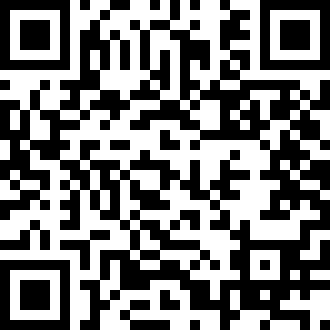
\includegraphics[width=\textwidth]{images/qr2.png}
    \caption{~}
    \label{Pic_QR_BW}
  \end{subfigure}
  \hfill
  \begin{subfigure}[b]{0.45\textwidth}
    \centering
    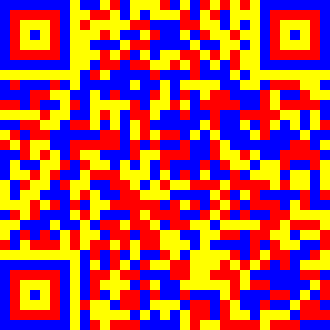
\includegraphics[width=\textwidth]{images/qr3.png}
    \caption{~}
    \label{Pic_QR_Color}
  \end{subfigure}
  \caption{На QR коді ми можемо на власні очі побачити біти (а); також показаний гіпотетичний QR код, який складається зі тритів (б).}
  \label{PicQR}
\end{figure}

Але я б хотів виділити один момент, який буде для нас важливим.
Інформація це часто є акцентування однієї з можливих альтернатив.
Наприклад, «Танєєв народився у 1856 році».\footnote{
  Приклад про Танєєва взятий з оповідання Іраклія Андронікова «Перший раз на естраді», яке можна прочитати в інтернеті або подивитися на youtube.
  \par\url{https://www.youtube.com/watch?v=dm8wdFKag94}}
Це означає, що Танєєв не міг народитися у 1858 році, 1859, 1860, 1861, 1862, і т.~д.
Тобто з усіх можливих альтернатив, коли міг народитися Танєєв, ми обираємо одну.
Цього погляду нам вистачить для потреб цієї книги.

Добре, тепер спробуємо поміркувати так, як це роблять програмісти та математики.
Який шмат інформації самий найпростіший?
Інтуїтивно, це вибір однієї з двох альтернатив.
Тому що три це вже забагато, а у разі однієї альтернативи мова не йде про вибір.
«Танєєв народився від батька та матері!»
Це викликає посмішку, бо незрозуміло, які є ще варіанти?
Так, з сучасними технологічними досягненнями у галузі біомедицини, у певному контексті ще можна уявити на чому саме робиться акцент, але не у 1856 році.

Сама дрібна одиниця інформація, а саме вибір однієї з двох альтернатив, називається бітом. \index{біт}
Це може бути орел чи решка, парне або непарне, біле або чорне, хрестик або нулик, \Male\ або \Female, живий або мертвий, уперед чи назад, правда чи брехня.

\begin{exercise}
Придумайте ще приклади інформації, які можна закодувати одним бітом.
\end{exercise}

У сучасній мікроелектроніці, біт це наявність або відсутність електричного сигналу за певний проміжок часу, який називається тактом. \index{такт}
Переважна кількість сучасних процесорів бачать увесь свій світ виключно як послідовність біт.
Коли ми на комп'ютері слухаємо музику, дивимося відео або граємо у 3D ігри, коли робиться автоматичний переклад з однієї мови на іншу, коли автоматично генеруються пейзажі, то інколи дуже важко повірити в те, що віртуальна реальність складається виключно з бітів, але це так.
Однією нашою метою буде як раз пояснення того, як реальний світ може бути змодельований з бітів.

Проте, поширення електронних пристроїв призвело до того, що ми можемо фізично побачити біти навіть у реальному житті.
Гарний приклад цього це QR~коди, де біти видно на власні очі (рис.~\ref{Pic_QR_BW}).
Тут чорні квадратики кодують один стан, а білі---інший.

Оскільки ми будемо вести багато розмов про біти, було б добре їх якось позначати.
Біт може бути у одному з двох станів, тому для цього можна вибрати два будь-яких символи, наприклад $\blacksquare$ та $\square$, як на QR~коді.
Але історично в математиці для цього використовуються числа $0$ та $1$.
Щоб відрізняти звичайні десяткові числа, складені з нулів та одиниць, наприклад, як  $101$ (сто один),  від послідовності біт \bitstr{1}, \bitstr{0} та \bitstr{1}, ми будемо триматися наступних домовленостей:
\bitdesc

За визначенням, один біт може кодувати два різних варіанти. А скільки варіантів кодує два біти? Нескладно порахувати, що відповідь на це запитання буде чотири, ось усі варіанти: \bitstr{00}, \bitstr{01}, \bitstr{10} та \bitstr{11}. Взагалі, якщо ми збільшуємо кількість біт на один, то кількість варіантів зростає у двічі.
Це легко пояснити тим, що для будь якого попередньої комбінації ми можемо додати або біт \bitstr{0}, або біт \bitstr{1}.
Загально, якщо в нас є $n$ біт, то з них можна скласти $2^n$ різних комбінацій.

\begin{exercise}
Побудуйте усі різні комбінації, які можна створити з трьох біт.
\end{exercise}

\begin{exercise}
Скільки усього можливих комбінацій можна скласти з $10$ біт?
\end{exercise}

Я сподіваюся, що до цього моменту ви вже розібралися, що таке біти.
Тому настав час трохи відпочити та пофлудити.
Отже, біт має два стани, які ми позначаємо \bitstr{0} та \bitstr{1}.
Також ми відмітили, що безглуздо розглядати щось, що має лише один стан.
А якщо розглянути систему, яка має три стани, наприклад \tritzero, \tritone\ та \trithalf?
\index{тріт} Назвемо трітом одиницю інформації, де у нас є вибір з трьох альтернатив.

\begin{exercise}
Побудуйте усі різні комбінації, які можна створити з двох тритів.
\end{exercise}

Чи дасть це нам якісь переваги?
З математичної точки зору, усе що можна представити з тритів, можна представити й за допомогою бітів.
Самий простий шлях це зробити просто використовувати два біти для кодування одного тріта: \bitstr{00}~—~\tritzero, \bitstr{11}~—~\tritone\ та \bitstr{01}~—~\trithalf.
Так, звичайно комбінація \bitstr{10} не буде використовуватися.
Так, звичайно бітів буде вдвічі більше ніж тритів.
Але коли це хвилювало математиків?

\begin{exercise}
Скільки біт треба для того, щоб закодувати інформацію, яка міститься у двох трітах?
Скільки комбінацій при цьому не буде використано?
\end{exercise}

Добре, а що з точки зору народного господарства?
Якщо зберігати інформацію у трітах замість бітів, чи не виграємо ми додаткове місце?
Яке не яке, а досягнення.
Але, на практиці усе не так просто.
Безкоштовний газ є тільки у газовій камері.

Подивимося на рис.~\ref{Pic_QR_Color}.
На ньому я намагався нафантазувати, як би мав виглядати QR~код з тритів.
Замість чорної та білої фарб, використано жовту, синю та червоні фарби.
Ніби то виграш є?
Але на практиці розрізняти три фарби складніше.
Тому у звичайному чорно-білому варіанті ми зможемо розрізняти менші квадратики, а це також буде впливати на щільність запису інформацію.

Зробити процесори, які працюють з трітами, не питання.
За радянських часів була побудована ЕОМ Сетунь\footnote{\setunref}, яка працювала з трітами. \index{Сетунь}
Розрізнялися не тільки наявність та відсутність сигналу, але й його напрямок.
Хтось й по сьогоднішній день вважає це революційним досягненням, але я до цього ставлюся скептично.
Проектування процесорів зараз суто технічний процес.
Е багато інструментів, програмних застосунків, які дозволяють моделювати нові процесори.
Цим займається багато спеціалістів по усьому світу, тому усе що можна було перепробувати, вони вже перепробували.
Отже, якщо переважна більшість сучасних комп'ютерів працюють з бітами, то це означає, що не зважаючи на свою привабливість, тріти все ж таки програють бітам.

Але, там де це доречно, то чому б не розглянути?
У WiFi інформація передається символами, кожен з яких може нести величезну кількість варіантів.
Так, оскільки ця інформація у евентуально буде оброблятися звичайним процесором, то з практичної точки зору цю кількість варіантів намагаються зробити ступенями двійки.
Це дає змогу казати, що один символ несе $1024$ біти інформації.
Але у самій електромагнітній хвилі важко побачити окремі біти.

Також скажу декілька слів про квантові обчислення, кубіти, або квантові біти. \index{кубіт}
Так, на сьогодні віртуальний світ складається з бітів. А що у реальному?
Якщо опуститися на рівень квантових взаємодій, ми побачимо, що там працюють свої екзотичні контрінтуїтивні закони.
Окрім двох альтернатив, які виключають одна одну, ми часто бачимо їх суперпозицію.
Наприклад, електрон на $30$\% обертається праворуч, а на $70$\%---ліворуч.
Нам це важко уявити, але математичні формули працюють саме так.
Замість нуля та одиниці, ми отримуємо фізичну величину від нуля до одиниці.
Додайте ще фазу від нуля до $2\pi$, й ви отримаєте кубіт.
А ще суперпозиція станів, зворотні операції, вимірювання...

Вже з'являються перші квантові комп'ютери, які оперують кубітами.
Це може бути новою революцією.
Але на початку все ж таки краще освоїти звичайне програмування, яке працює з бітами.
А вже потім переходити до квантового.

\begin{exercise}
Продивиться статтю у Wikiepedia про квантові комп'ютери\footnote{\quantumref}. Чи це цікаво?
\end{exercise}

\begin{summary}
\item Інформація вимірюється у бітах.  Біт це найменший шмат інформації, який складається з двох станів, які позначаються \bitstr{0} та \bitstr{1}.
\item З $n$ біт можна скласти $2^n$ різних комбінацій.
\end{summary}

\printindex
\end{document}
